\documentclass[12pt,letterpaper]{article}

\usepackage{amsmath}
%\usepackage[margin=1.3in]{geometry}
\usepackage[pdftex]{graphicx}
\usepackage{hyperref} 

\parindent 0cm

\graphicspath{{figures/}}

\author{
    Jed Barlow\\
    \textit{ejbarlow@ualberta.ca}
}
\title{SeqPartitioner Geneious Plugin Manual}

\begin{document}
\maketitle

\hfill

%\newpage
\tableofcontents

\newpage
\section{Overview}

SeqPartitioner is a Geneious plugin for partitioning allele multisets.  The
plugin operates on alignments to produce various tables expressing the grouping
of equivalent aligned nucleotide sequences and the number of differences
between strains in terms of non-equivalent alleles.

\section{Installation}
The plugin can be obtained, at the time of the writing of this manual, from two
locations.

\begin{itemize}
\item
    In source form: \url{http://github.com/jedbarlow/biol398\_seq\_partitioner/}
\item
    As a compiled package: \url{http://www.ualberta.ca/~ejbarlow/biol398/}
\end{itemize}

Once obtained, the plugin \textit{SeqPartitioner.gplugin} can be installed by
navigating the Geneious menu to \texttt{Tools->Plugins}.

\hfill

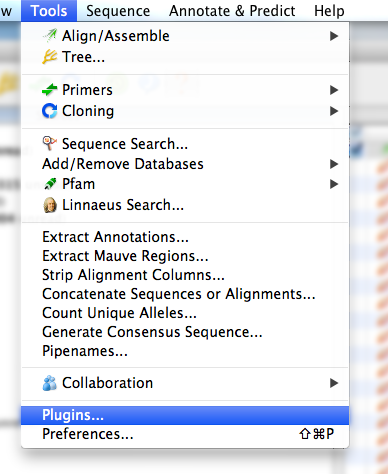
\includegraphics[resolution=130]{menu_entry_plugins.png}

\hfill

Then pressing the \texttt{Install plugin from a gplugin file...} button.

\hfill

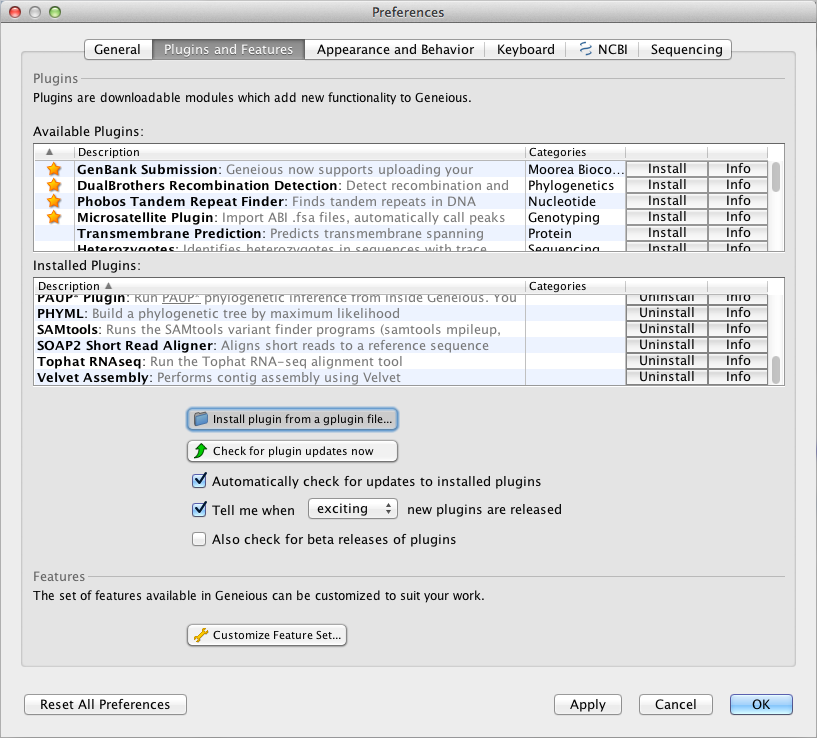
\includegraphics[resolution=130]{plugins_dialog.png}

\hfill

Finally, navigate to and select the plugin package file
\textit{SeqPartitioner.gplugin}.

Once installed, an entry should appear in the Geneious menu as shown in the
second figure below.

\section{Operation}
The plugin is used by first selecting a set of alignments.

\hfill

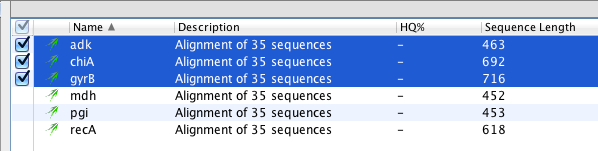
\includegraphics[resolution=120]{alignment_selection.png}

\hfill

Then navigating the menu to \texttt{Tools->Partition Allele Multiset}.


\hfill

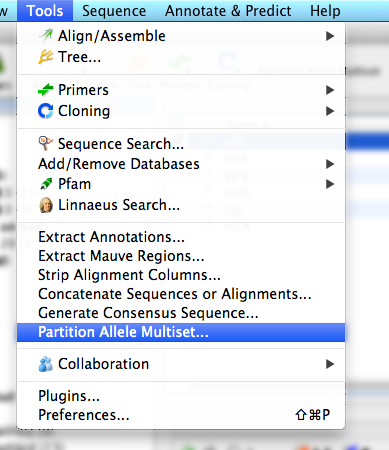
\includegraphics[resolution=130]{menu_entry.png}

\hfill

Then choosing options in the dialog box.

\hfill

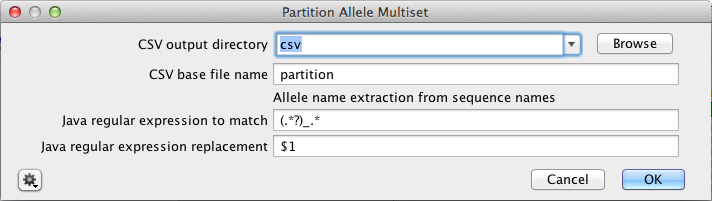
\includegraphics[resolution=130]{dialog_box.png}

\hfill

The meanings of the fields are as follows:

\begin{itemize}
\item \textit{CSV output directory} \hfill \\
\addcontentsline{toc}{subsubsection}{CSV output directory}
    This is the target directory into which the resulting table files will be
    written.  Note that pre-existing files of the same name as the output files
    will be overwritten without confirmation.

\item \textit{CSV base file name} \hfill \\
\addcontentsline{toc}{subsubsection}{CSV base file name}
    This is a string of text which will be appended with descriptive suffixes
    for each table.  For example the following entry,
    
    \begin{itemize}
    \item[]\texttt{partition1}
    \end{itemize}

    will result in the production of the following files,

    \begin{itemize}
    \item[]\texttt{partition1\_gene\_vs\_strain.csv}
    \item[]\texttt{partition1\_strain\_vs\_strain.csv}
    \item[]\texttt{partition1\_strain\_vs\_strain\_matrix.csv}
    \end{itemize}

\item \textit{Java regular expression pattern match} \hfill \\
\addcontentsline{toc}{subsubsection}{Java regular expression pattern match}
    The purpose of these last two fields is to establish a transformation of
    sequence names to the strain names, so that strains can be correlated
    between alignment files.  The first field is a pattern to match against
    each sequence name.

\item \textit{Java regular expression replacement} \hfill \\
\addcontentsline{toc}{subsubsection}{Java regular expression replacement}
    This field describes a replacement for the text in the sequence name
    matched by the pattern in the previous field.

\end{itemize}

\subsection{Example Regular Expressions}

\begin{itemize}
\item
    If for example, the names of the sequences are patterned as
    \texttt{STRAIN\_GENE}, then the default entry will work correctly by
    reducing sequence names to strain names, which will be consistent across
    alignment files and allow for correlation.

    Pattern: \texttt{(.*?)\_.*}

    Replacement: \texttt{\$1}

    The period matches any character, and the star matches a sequence of
    characters matching the previous construct (the period in this case).  The
    question mark indicates that the star should only match until the next
    construct (an underscore in this case) can be matched.  The parenthesis in
    the pattern designate the inner matching text as an identifiable string
    which can be referred to in the replacement as \texttt{\$1}.  It is
    important to note that text in the sequence name which does not match the
    pattern will be left unmodified, so the last part of the pattern
    \texttt{\_.*}, which matches the \texttt{\_GENE} portion of the name,
    cannot be omitted.

\item
    Sequence names patterned such as \texttt{GENE\_STRAIN} can be properly
    grouped by slightly modifying the pattern in the above.

    Pattern: \texttt{.*?\_(.*)}

    Replacement: \texttt{\$1}

\end{itemize}

More information about regular expressions, and in particular Java regular
expressions, can be found at the following urls.

\begin{itemize}
\item
    \url{https://en.wikipedia.org/wiki/Regular\_expression}
\item
    \url{http://docs.oracle.com/javase/tutorial/essential/regex/intro.html}
\item
    \url{http://docs.oracle.com/javase/7/docs/api/java/util/regex/Pattern.html}
\end{itemize}

\newpage
\section{Description of Output Tables}
%\parindent 15pt
\parskip 10pt

Two tables are created when the plugin is run.  The tables with the suffixes
\texttt{straing\_vs\_strain} and \texttt{straing\_vs\_strain\_matrix}
describe the number of different alleles (according to the equivalence
relation) between any two strains.

The table with the suffix \texttt{gene\_vs\_strain} contains a column for each
gene (alignment file), and a row for each strain.  The number in a row
indicates which group that allele matches with respect to other alleles of
strains in the same column.  The final column on the right indicates a
partitioning of the rows of the other columns, so each matching row of numbers
in the other columns will have the same value in the right most column.

\subsection{Partition Relation and Errors}
The equivalence relation used for partitioning is a comparison of aligned
nucleotide sequences where `-' is always considered a match with the
corresponding character in the other sequence.  As a consequence, transitivity
of the equivalence relation can break under certain conditions.  So, for
example, the following sequences cannot be partitioned:

\parskip 0cm
\begin{enumerate}
\item[(1)] ATC
\item[(2)] A-C
\item[(3)] AGC
\end{enumerate}

\parskip 10pt

Since we have $(\texttt{1}) = (\texttt{2}) = (\texttt{3})$, but $(\texttt{1})
\ne (\texttt{3})$, therefore no partition can be formed which both groups equal
sequences and separates unequal sequences.

When such an error occurs, there will be entries of \texttt{-1} in the
resulting table.  Such values may not be the most effective indicators to use
for identifying the source sequences of the error, because the situations of
overlapping groups may be very complex and not comprehensively identified by
the error markings.  No table results should be accepted if the table contains
a \texttt{-1}.

\end{document}


% Each alignment file is assumed to contain sequences pertaining to exactly one
% gene, and it is assumed that each gene has all it's sequences in one
% alignment file.

% The purpose of the regexp is to enable strains to be correlated accross
% alignment files
